% ============================================================
% Figure 8: Ablation Study — Contribution of Each Component
% ============================================================
\documentclass[border=5pt]{standalone}
\usepackage[T1]{fontenc}
\usepackage{pgfplots}
\pgfplotsset{compat=1.18}

\definecolor{cb1}{RGB}{0,101,189}
\definecolor{cb2}{RGB}{204,51,51}
\definecolor{cb3}{RGB}{0,128,0}
\definecolor{cb4}{RGB}{230,159,0}
\definecolor{cb5}{RGB}{117,112,179}

\begin{document}
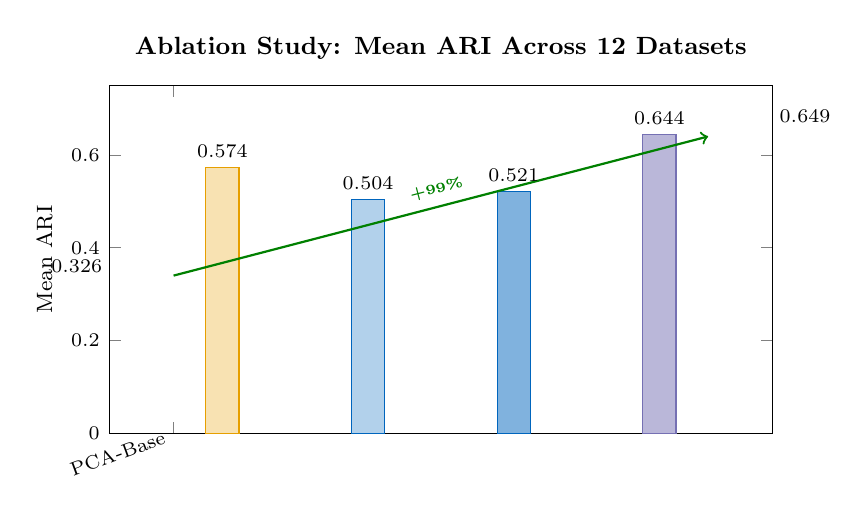
\begin{tikzpicture}
\begin{axis}[
    width=10cm, height=6cm,
    ybar,
    bar width=12pt,
    font=\footnotesize,
    title style={font=\small\bfseries},
    title={Ablation Study: Mean ARI Across 12 Datasets},
    symbolic x coords={PCA-Base, UMAP-Base, PCA+DE, UMAP+DE, EMR-CGC, DEAC},
    xtick=data,
    x tick label style={rotate=20, anchor=east, font=\scriptsize},
    ylabel={Mean ARI},
    ylabel style={font=\footnotesize},
    ymin=0, ymax=0.75,
    tick align=inside,
    tick label style={font=\scriptsize},
    grid=none,
    nodes near coords,
    nodes near coords style={font=\scriptsize\bfseries, above},
    every node near coord/.append style={/pgf/number format/.cd, fixed, precision=3},
    enlarge x limits=0.12,
]

\addplot[fill=cb2!30, draw=cb2] coordinates {(PCA-Base, 0.326)};
\addplot[fill=cb4!30, draw=cb4] coordinates {(UMAP-Base, 0.574)};
\addplot[fill=cb1!30, draw=cb1] coordinates {(PCA+DE, 0.504)};
\addplot[fill=cb1!50, draw=cb1] coordinates {(UMAP+DE, 0.521)};
\addplot[fill=cb5!50, draw=cb5] coordinates {(EMR-CGC, 0.644)};
\addplot[fill=cb3!50, draw=cb3] coordinates {(DEAC, 0.649)};

% Improvement annotations
\draw[->, cb3, line width=0.8pt] (axis cs:PCA-Base, 0.34) -- (axis cs:DEAC, 0.64)
    node[midway, above, font=\tiny\bfseries, cb3, sloped] {+99\%};

\end{axis}
\end{tikzpicture}
\end{document}
